%#!platex master-ohp.tex
\documentclass{slides}
\input{predef}

\begin{document}

$U(\infty)$$B$NBP>N@-$r2u$7$F$7$^$&!#(B\\
$\Rightarrow U(1)$$B%2!<%8>l$rF3F~$9$k$H(B$U(\infty)$$B$,I|3h!#(B

$\color{blue}x,y$$B$,$b$O$d8r49$7$J$$$N$G!"(B$\color{blue}x,y$$B$G1i;;;R7A<0$G(B
$B=q$$$?%O%_%k%H%K%"%s$O!"(B
\[\color{blue}
  \Ham=2\pi\Tr\left(\1half([\aniC,\creC]+1)^2
		 +[\aniC,\phi][\creC,\phi]
		 +\theta V(\phi)\right)
\]
\[\color{blue}
 \creC\equiv \crea+i\theta^{\1half}A,\quad
  \aniC\equiv \anih-i\theta^{\1half}\Ab\quad\mbox{($B6&JQHyJ,(B)}
\]
$B$3$3$G!"(B$U(\infty)$$B$NBP>N@-$,$"$k$H!"(B{\color{red} Solution generating
technique}$B$r;H$&$3$H$,$G$-$k!#$D$^$j0J2<$N$h$&$JJQ49$r$9$k$H!"(B
\underline{\color{blue} $B?7$7$$2r$r9=@.$G$-$k!#(B}
\[\color{blue}
 C\rightarrow SC\Sd,\quad\phi\rightarrow S\phi\Sd
\]
$B$3$3$G!"(B$S$$B$O(B{\color{red} isometry}$B$D$^$j!"(B\ovalbox{\color{blue}$\Sd
S=1$}$B$rK~$?$9!#(B\\
$BNc$($P(B$S$$B$,(Bshift operator \ovalbox{\color{blue}$S\equiv
\sum\limits_{k=0}^\infty \ket{k+1}\bra{k}$}$B$N;~(B
\[\color{blue}
 \left\{\begin{array}{l}
  \phi=\phi_*\\
  A=0\\
  E=0
 \end{array}\right.\mbox{\shortstack[c]{$S^n$\\ $\Rightarrow$}}
 \left\{\begin{array}{l}
  \phi=\phi_*(1-\sum\limits^{n-1}_{k=0}\ket{k}\bra{k}) \\
  \aniC=S^n\crea\Sd^n,\,\creC=S^n\anih\Sd^n \\
  E=2\pi n\left(\frac{1}{2\theta}+\theta V(0)\right)
 \end{array}\right.
\]

\newpage
%%%%%%%%%%%%%%%%%%%%%%%%%%%%%%%%%%%%%%%%%%%%%%%%%%%%%%%%%%%%%%%%%%%%%%%%

\begin{center}
 $B%?%-%*%s>l$N%]%F%s%7%c%k(B
 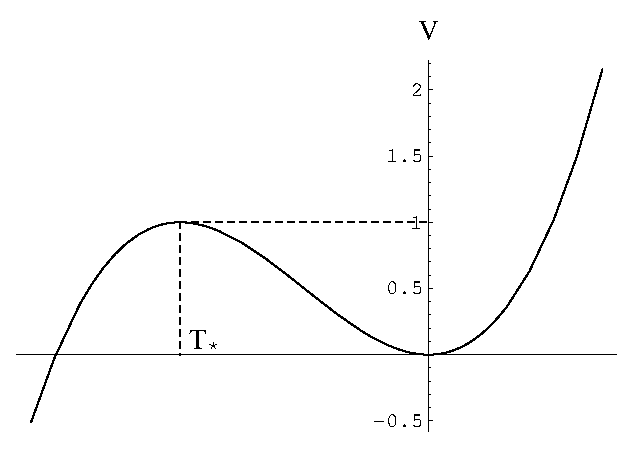
\includegraphics{tachyon-potential.eps}
\end{center}\vspace{-1cm}
Sen$B$N2>@b$K$h$k$H!"IT0BDj$J%?%-%*%s$N$"$k??6u$H%?%-%*%s$NL5$$??6u$H$N%?(B
$B%-%*%s%]%F%s%7%c%k$N:9$O(Bbrane$B$N%F%s%7%g%s$K0lCW$9$k!#(B\\
$\Rightarrow$\parbox{14cm}{$B%?%-%*%s>l$G(B\NCS $B$r9=@.$9$k$H(B,\\
\underline{\color{blue}$B$=$N%F%s%7%g%s$O(BD-brane$B$H0lCW$9$k!#(B}
$B2?8N$J$i$P!"(B2$B<!85$NJ}8~$r(B$\color{blue}$}


$B$5$i$K!"(B\NCS $B2r$N$^$o$j$N%2!<%8>l$N(Bfluctuation$B$r9M$($k$H!"(B\NCS $B$H%2!<%8(B
$B>l$N%+%C%W%j%s%0$N;EJ}$O(B\underline{\color{blue} D-brane$B$N$=$l$H0lCW$9$k!#(B}

$B0J>e$N;v<B$+$i<!$N$3$H$,8@$($=$&!#(B\\
\ovalbox{\parbox{16cm}{\color{blue} \NCS $B$O<B$O(BD-brane$B$rI=(B
$B$o$7$F$$$k!#(B}}

%%%%%%%%%%%%%%%%%%%%%%%%%%%%%%%%%%%%%%%%%%%%%%%%%%%%%%%%%%%%%%%%%%%%%%%

\typeout{=== Region from (point) to (mark) ===}

\end{document}
